
\section{Основные свойства Солнечной системы. Законы Кеплера}

Характерные размеры, числа, основные структуры Солнечной системы(СС). Вывод законов Кеплера.

\subsection{Структура СС. Характерные размеры}

Вокруг Солнца вращается целый комплекс объектов. Основная масса СС приходится на Солнце - его масса ~1.99$\cdot 10^{33}$ г., что составляет 99.86\% от массы СС.

Можно поделить СС на 5 основных групп(\textit{расположены в порядке удаления от Солнца}):

\begin{itemize}
	\item Планеты земной группы
	\item Пояс астероидов
	\item Планеты-гиганты
	\item Пояс Койпера
	\item (Рассеянный диск, о котором Попов совершенно не пишет в презентации)
	\item Облако Оорта
\end{itemize}

\subsubsection{Состав групп. Масштабы}

Деление на группы произведено по расстоянию и по типу объектов, входящих в состав группы. Из неочевидного, объекты пояса астероидов состоят в основном из горных пород и металлов; Здесь расположена одна из карликовых планет - Церера.

Объекты пояса Койпера же состоят в основном из летучих веществ(льдов) - метана, аммиака и воды, таким образом являясь возможным источником короткопериодических комет(например, комета Галлея с периодом 75-76 лет). Здесь расположены 4 оставшиеся карликовые планеты: Плутон, Эрида, Макемаке и Хаумеа.

Дальше идет Рассеянный диск, который содержит в себе такие же объекты, как и пояс Койпера, пересекаясь с последним, но простирается гораздо дальше от Солнца, и гораздо выше и ниже плоскости эклиптики.

Облако Оорта - это сферическая область СС, служащая источником долгопериодических планет, внешняя граница которой определяет гравитационную границу СС - на расстоянии около 2 св. лет.

Удобно для описания выражать расстояния до Солнца через \textbf{астрономическую единицу(a.u. или au)} - по определению, это(в приближении круговой орбиты) примерное расстояние от Солнца до Земли:

\begin{equation}
1 \text{ au} = 149 597 870 700 \text{ м.} \approx 150 \text{ млн. км.}
\label{eq:3_au}
\end{equation}

Тогда планеты земной группы - Меркурий, Венера, Земля, Марс - имеют орбиты ~0.3-0.47 au, ~0.71 au, ~1 au, ~1.38-1.67 au соответственно(интервалы - от наименьшего расстоянию(в перигелии) до Солнца, до наибольшего(в афелии)).

(Главный) пояс астероидов лежит в пределах ~2.06-3.27 au.

Планеты-гиганты - Юпитер, Сатурн, Уран, Нептун - имеют орбиты ~4.95-5.45 au, ~9-10.1 au, ~18.4-20.1, ~29.8-30.4 соответственно.

Пояс Койпера располагается на ~35-50 au от Солнца, Рассеянный диск на ~45-100 au(поэтому Эриду иногда причисляют именно к этому диску, потому что хоть и перигелий лежит в Поясе Койпера, большая полуось орбиты равна ~67.7 au).

Внешняя граница облака Оорта, по разным оценкам, составляет от 50000 до 200000 au.

\subsubsection{Размеры объектов}

Удобно для описания размеров планет и спутников использовать средний радиус Земли:

\begin{equation}
R_{\oplus} \approx 6371 \text{ км.}
\label{eq:3_r_earth}
\end{equation}

Для остального пользуемся старыми-добрыми км.

Основные элементы групп:

\begin{itemize}
	\item Планеты(о них следующий билет)
	\item Спутники - размеры от нескольких километров, до крупнейшего спутника Юпитера, имеющего радиус 0.413 земных.
	\item Планеты-карлики - объекты округлой формы, диаметром 400-2500 км.
	\item Астероиды - объекты неправильной формы, диаметром 1-1000 км.
	\item Кометы - объекты радиусом 1 - 10 км.
\end{itemize}

\subsection{Законы Кеплера}

Кеплер вывел эти 3 закона, вручную проанализировав огромное количество наблюдений. Их формулировка:


\begin{enumerate}
	\item Орбиты планет эллиптические, Солнце находится в одном из фокусов.
	\item Планета всегда заметает радиус-вектором одинаковую площадь за одинаковое время.
	\item Квадраты периодов(время, за которое планета проходит орбиту) относятся как кубы больших полуосей данных орбит.
\end{enumerate}

\begin{figure}[H]
	\centering
	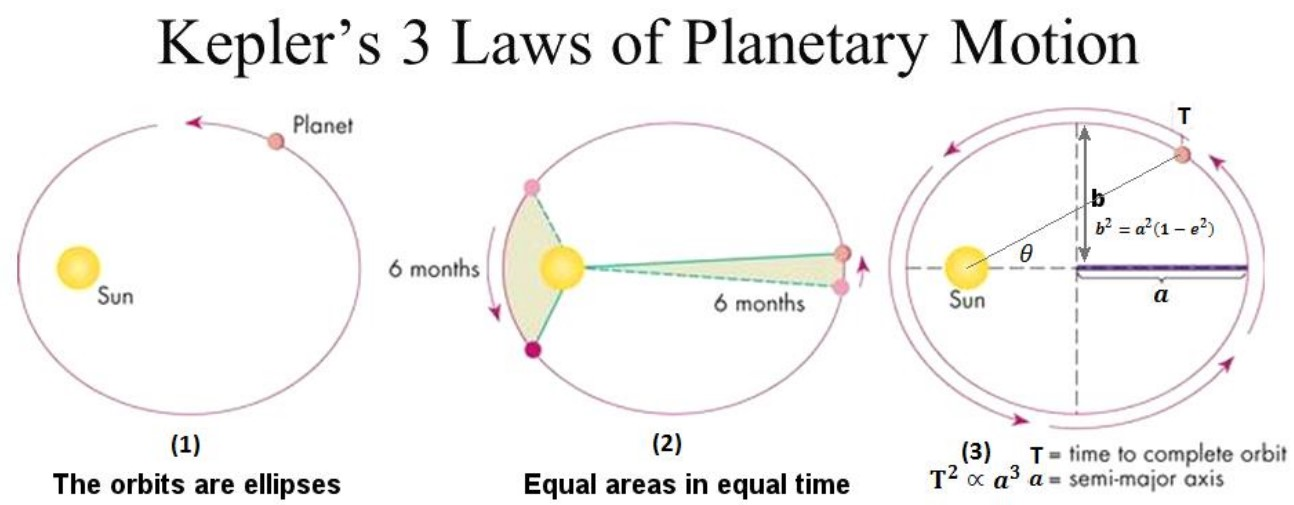
\includegraphics[width=0.7\linewidth]{3_kepler_laws}
	\caption{Графическое определение законов Кеплера}
	\label{fig:3_kepler_laws}
\end{figure}

\subsubsection{Подробнее о каждом законе}

Почему эллипсы? Ответ следует из закона сохранения энергии. Если еще и вспомнить, что сохраняется орбитальный момент L, то вывод упрощается:

\begin{figure}[H]
	\begin{subfigure}
		\centering
		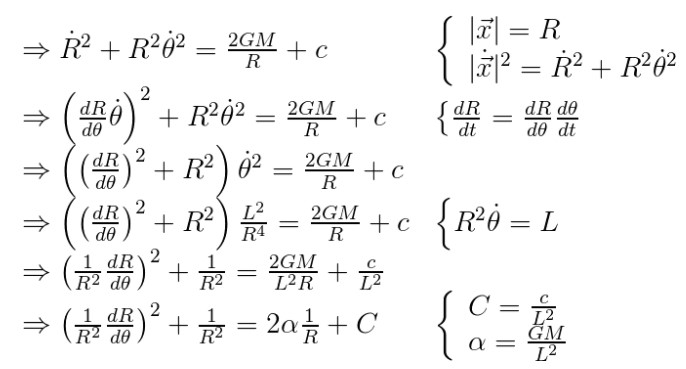
\includegraphics[width=0.7\linewidth]{3_ellipse_first}
	\end{subfigure}
	
	\begin{subfigure}
		\centering
		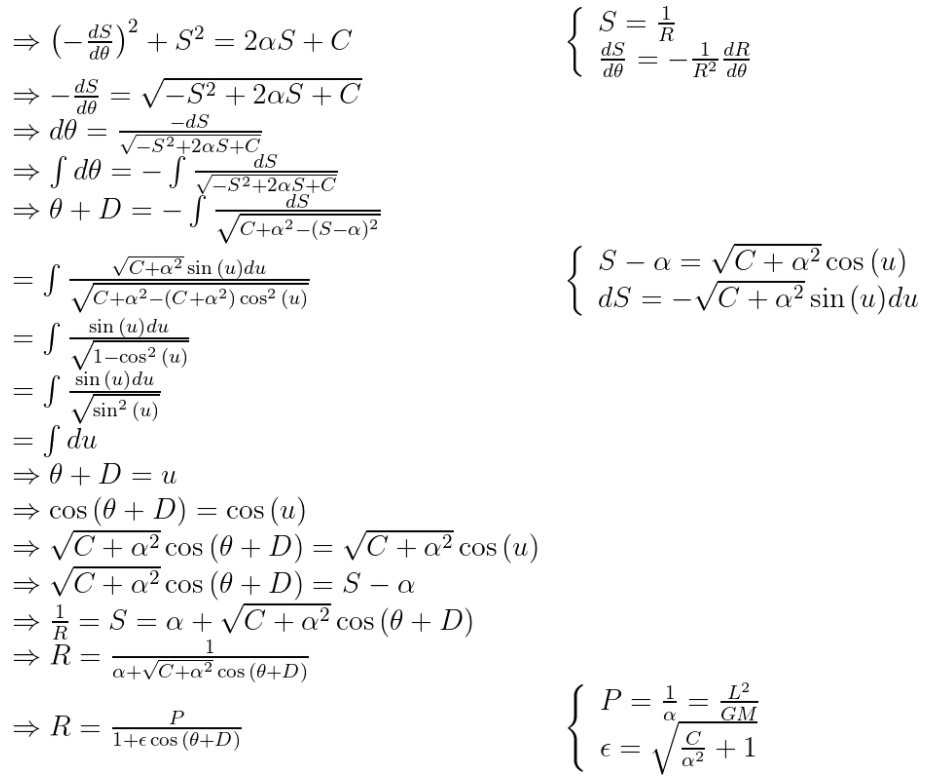
\includegraphics[width=0.7\linewidth]{3_ellipse_second}
	\end{subfigure}
	
	\caption{Связь радиуса и угла для эллиптической орбиты}
	\label{fig:3_ellipse}
\end{figure}

\textbf{Размер} большой полуоси зависит от полной энергии E, \textbf{форма(эксцентриситет)} - от орбитального момента L.

Второй закон - следствие сохранения орбитального момента:

\begin{eqnarray}
L = M_{pl} \cdot [\vec{r} \times \vec{V}] = const, \implies [\vec{r} \times \vec{V}] = const 
\label{eq:3_orb_moment}
\\
\text{Заметаемая площадь } \vec{dS} = [\vec{r} \times \vec{V}] dt, \implies \frac{\vec{dS}}{dt} = const
\label{eq:3_kepler_area}
\end{eqnarray}

Физическое следствие из этого - в ближайшей точке орбиты скорость тела наибольшая.

Третий закон можно вывести из второго закона Ньютона для притяжения тела к звезде, но является следствием закона сохранения энергии. Решая задачу двух тел и переходя к приведенной массе(M - масса звезды, m - масса планеты):

\begin{eqnarray}
\mu = \frac{Mm}{M + m}
\label{eq:3_reduced_mass}
\\
\frac{ \mu v^2 }{2 a} = \frac{GMm}{a^2}, v = \frac{2 \pi a}{P}, \text{считаем что $a_{st} \ll a_{pl} = a$}
\label{eq:3_newton}
\\
\implies P^2 = \frac{4 \pi^2}{G(M + m)} a^3 \text{ - уточнённая формулировка Третьего закона Кеплера}
\label{eq:3_kepler_third}
\end{eqnarray}

В приближении, что масса планеты много меньше массы звезды, можно пренебречь m в знаменателе и получится универсальная для звезды величина, связывающая период и большую полуось для орбит тел с маленькой массой, тем самым формулируя первоначальный(неточный) 3 закон Кеплера: "Квадраты периодов планет относятся как кубы больших полуосей".

